
We define the basic model; some extensions thereof are specified in  Section~\ref{sec:theory-extensions}.

\xhdr{Principals and agents.} There are two principals and $T$ agents,
denoted, resp., principal $i\in \{1,2\}$ and agent $t\in [T]$. The game proceeds in (global) rounds. In each round $t\in [T]$, the following  interaction takes place. Agent $t$ arrives and chooses a principal $i_t\in \{1,2\}$. The principal chooses action $a_t\in A$, where $A$ is a fixed set of actions (same for both principals and all rounds). The agent experiences this action, receives a reward $r_t\in \{ 0,1\}$, and reports it back to the principal. We posit \emph{stochastic rewards}: whenever a given action $a\in A$ is chosen, the reward is an independent draw from Bernoulli distribution with mean $\mu_a$. The mean rewards $\mu_a$ are initially not known to anybody. Each principal is completely unaware of the rounds when the other principal is chosen.

Each principal $i$ commits to a learning algorithm \alg[i] before round $1$, and uses this algorithm throughout. The algorithm follows the protocol of \emph{multi-armed bandits} (\emph{MAB}). Namely, it proceeds in time-steps:%
\footnote{These time-steps will sometimes be referred to as \emph{local steps/rounds}, so as to distinguish them from ``global rounds" defined before. We will omit the global vs. local distinction when clear from the context.} each time it is called, it outputs an action from $A$, and inputs a reward for this action. \alg[i] is called only in global rounds when principal $i$ is chosen.

\newcommand{\est}{\mathtt{est}}

\xhdr{Agents' response.} Each agent $t$ forms a reward estimate $\est_i(t)$ for each principal $i$, as specified below, and chooses the principal based on these reward estimates. Specifically, principal $1$ is chosen with probability
\begin{align}
p_t = \respF\rbr{ \est_1(t) - \est_2(t) },
\end{align}
where $\respF:[-1,1]\to [0,1]$ is the \emph{response function}, same for all agents and known to everyone.

We assume that $\respF$ is monotonically non-decreasing, is larger than $\nicefrac12$ on the interval $(0,1]$, and smaller than $\nicefrac12$ on the interval $[-1,0)$. We consider three specific models (see \reffig{fig:response-functions}):

\begin{figure}
\begin{center}
  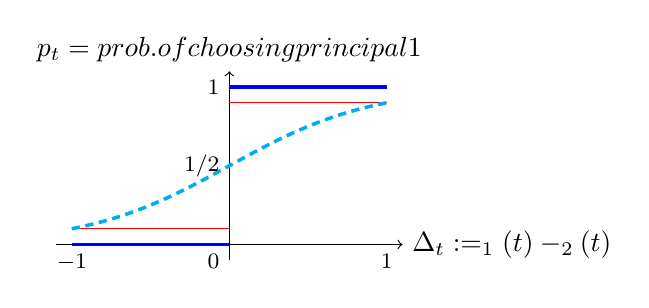
\begin{tikzpicture}[scale=2.0]
    \draw[->] (-1.1,0) -- (1.1,0) node[right]
    {$\Delta_t := \est_1(t) - \est_2(t)$};
    \draw[->] (0,-0.1) -- (0,1.1) node[above]
        {$p_t = \text{prob. of choosing principal 1}$};
    \draw[scale=1.0,domain=-1:0,smooth,variable=\q,blue, line width=0.50mm] plot ({\q},{0});
    \draw[scale=1.0,domain=0:1,smooth,variable=\q,blue,line width=0.50mm] plot ({\q},{1});
    \draw[scale=1.0,domain=-1:0,smooth,variable=\y,red]  plot ({\y},{0.1});
    \draw[scale=1.0,domain=0:1,smooth,variable=\y,red]  plot ({\y},{0.9});
    \draw[scale=1.0,domain=-1:1,smooth,variable=\y,cyan, line width=0.45mm, dash pattern=on 3pt off 2pt]  plot ({\y},{1/(1 + 1/(9^\y))});
    % \node[above, blue] at (0.5, 0.5) {\footnotesize $2 q (1 - q)$};
     \node[left] at (0, 0.5) {\footnotesize $1/2$};
     \node[left] at (0, 1) {\footnotesize $1$};
     \node[below left] at (0, 0) {\footnotesize $0$};
     \node[below ] at (1, 0) {\footnotesize $1$};
     \node[below ] at (-1, 0) {\footnotesize $-1$};
  \end{tikzpicture}
\end{center}
\caption{The three models for $\respF$: \HardMax is thick blue, \HardMaxRandom is slim red, and \SoftMaxRandom is the dashed curve.}
\label{fig:response-functions}
\end{figure}

\begin{itemize}
\item \HardMax: $\respF$ equals $0$ on the interval $[-1,0)$ and $1$
  on the interval $(0,1]$. In words, a \HardMax agent
  deterministically chooses a principal with a higher reward estimate.

\item \HardMaxRandom:
    % $\respF$ equals $\eps$ on the interval $[-1,0)$ and $1-\eps'$ on the interval $(0,1]$, where $\eps,\eps'\in (0,\tfrac12)$ are some positive constants. In words, each agent is a \HardMax agent with probability $1-\eps-\eps'$, and with the remaining probability she makes a random choice.
    $\respF$ equals $\eps_0$ on the interval $[-1,0)$ and $1-\eps_0$ on the interval $(0,1]$, for some constant $\eps_0\in (0,\tfrac12)$. In words, each agent is a \HardMax agent with probability $1-2\eps_0$, and makes a random choice otherwise.


\item \SoftMaxRandom: $\respF(\cdot)$ is bounded away from $0$ and $1$, and ``smooth" around $0$ (see Section~\ref{sec:theory-SoftMax}).
\end{itemize}
% \asedit{(We assume $\respF(-1)+\respF(1)=1$ in \HardMaxRandom and \SoftMaxRandom only to simplify notation.)}


%We say that $\respF$ is \emph{symmetric} if $\respF(-x)+\respF(x)=1$ for any $x\in [0,1]$. This implies \emph{fair tie-breaking}: $\respF(0)=\tfrac12$.

\xhdr{The \TheoryModel.}
In this model variant, the mean reward vector $\mu = (\mu_a:\; a\in A)$ is drawn from a common Bayesian prior $\priorMu$ before round $1$. Agents know the principals' algorithms. Their reward estimates are defined as Bayesian-expected rewards: for each agent $t$ and principal $i$,
\[ \est_i(t) := \E\sbr{ r_t\mid i_t = i }.\]


\ascomment{stopped here.}

with a common prior. More formally, for each action $a\in A$ there is a parametric family $\psi_a(\cdot)$ of
reward distributions, parameterized by the mean reward $\mu_a$. (The paradigmatic case is 0-1 rewards with a given expectation.) The
mean reward vector $\mu = (\mu_a:\; a\in A)$ is drawn from prior distribution $\priorMu$ before round $1$. Whenever a given action $a\in A$ is chosen, the reward is drawn independently from distribution $\psi_a(\mu_a)$. The prior $\priorMu$ and the distributions $(\psi_a(\cdot)\colon a\in A)$ constitute the (full) Bayesian prior on rewards, denoted $\prior$.



The information structure is as follows. The prior $\prior$ is known to everyone. The mean rewards $\mu_a$ are not revealed to anybody and each principal is completely unaware of the rounds when the other is chosen. We consider two variants of our model with different information structures. In the first, the  \textit{expectation choice} variant, each agent knows both principals' algorithms, and the global round when (s)he arrives, \emph{but not} the rewards of the previous agents. In the second, the \textit{reputation choice} variant, agents only make decisions based on the rewards of previous agents. Concretely, each of the two principals has a \emph{reputation score}, and each agent's choice is driven by these two numbers. The reputation score is simply a sliding window average: an average reward of the last $M$ agents that chose this firm.



Throughout, $\E[\cdot]$ denotes expectation over all applicable randomness.

\xhdr{Bayesian-expected rewards.}
Consider the performance of a given algorithm \alg[i], $i\in \{1,2\}$, when it is run in isolation (\ie without competition, just as a bandit algorithm). Let $\rew_i(n)$ denote its Bayesian-expected reward for the $n$-th step.

Now, going back to our game, fix global round $t$ and let $n_i(t)$ denote the number of global rounds before $t$ in which this principal is chosen. Then:
\begin{align*}
 \E[r_t \mid \text{principal $i$ is chosen in round $t$ and $n_i(t)=n$} ]
    = \rew_i(n+1) \quad (\forall n\in\N).
\end{align*}

\xhdr{Agents' response.}
Each agent $t$ chooses principal $i_t$ as follows: it chooses a distribution over the principals, and then draws independently from this distribution. Let $p_t$ be the probability of choosing principal $1$ according to this distribution. Below we specify $p_t$; we need to be careful so as to avoid a circular definition.

\gaedit{

The form of $p_t$ depends on the information structure that we consider.
In the expectation choice model, where the agents only know the global round and the principals' algorithms, it is defined as follows.

}

Let $\mI_t$ be the information available to agent $t$ before the
round. Assume $\mI_t$ suffices to form posteriors for quantities
$n_i(t)$, $i\in \{1,2\}$, denote them by $\posteriorN{i}{t}$. Note
that the Bayesian expected reward of each principal $i$ is a function
only of the number rounds he was chosen by the agents, so the
posterior mean reward for each principal $i$ can be written as
\begin{align*}
 \PMR_i(t) := \E[r_t \mid \text{$\mI_t$ and $i_t=i$} ]
    = \E[\rew_i(n_i(t)+1) \mid \mI_t]
    = \E_{n\sim \posteriorN{i}{t}}[\rew_i(n+1)].
\end{align*}
This quantity represents the posterior mean reward for principal $i$
at round $t$, according to information $\mI_t$; hence the notation \PMR. In general, probability $p_t$ is defined by the
posterior mean rewards $\PMR_i(t)$ for both principals. We assume a
somewhat more specific shape:
\begin{align}
p_t = \respF\left(\; \PMR_1(t) - \PMR_2(t) \;\right).
%p_t = \respF(\Delta_t), \quad \text{where } \Delta_t := \PMR_1(t) - \PMR_2(t).
\end{align}
Here $\respF:[-1,1]\to [0,1]$ is the \emph{response function}, which is the same for all agents. We assume that the response function is known to all agents.

To make the model well-defined, it remains to argue that information $\mI_t$ is indeed sufficient to form posteriors on $n_1(t)$ and $n_2(t)$. This can be easily seen using induction on $t$.

Since all agents arrive with identical information (other than knowing which global round they arrive in), it follows that all agents have identical posteriors for $n_{i,t}$ (for a given principal $i$ and a given global round $t$). This posterior is denoted $\posteriorN{i}{t}$.

\gaedit{
In the reputation choice variant we consider, at a given time $t$ each principal $i \in \{1, 2 \}$ has a reputation score denoted as $\REP_i (t)$. In this case we have that the agent's responses take an analogous form as in the first case:
\begin{align}
p_t = \respF\left(\; \REP_1(t) - \REP_2(t) \;\right).
\end{align}
}


\xhdr{MAB algorithms.}
We characterize the inherent quality of an MAB algorithm in terms of its \emph{Bayesian Instantaneous Regret} (henceforth, \BIR), a standard notion from machine learning:
\begin{align}
\BIR(n) := \E_{\mu\sim\priorMu}
    \left[ \max_{a\in A} \mu_a\right] - \rew(n),
\end{align}
where $\rew(n)$ is the Bayesian-expected reward of the algorithm for the $n$-th step, when the algorithm is run in isolation. We are primarily interested in how \BIR scales with $n$; we treat $K$, the number of arms, as a constant unless specified otherwise.

We will emphasize several specific algorithms or classes thereof:

\begin{itemize}
\item ``smart" MAB algorithms that combine exploration and exploitation, such as UCB1 \cite{bandits-ucb1} and \gaedit{Thompson Sampling \cite{russo2018tutorial}}. These algorithms achieve
        $\BIR(n) \leq  \tilde{O}(n^{-1/2})$
    for all priors and all (or all but a very few) steps $n$. This bound is known to be tight for any fixed $n$.\footnote{This follows from the lower-bound analysis in \cite{bandits-exp3}.}

\item ``naive" MAB algorithms that separate exploration and exploitation, such as Explore-then-Exploit and $\eps$-Greedy. These algorithms have dedicated rounds in which they explore by choosing an action uniformly at random. When these rounds are known in advance, the algorithm suffers constant \BIR in such rounds. When the ``exploration rounds" are instead randomly chosen by the algorithm, one can usually guarantee an inverse-polynomial upper bound \BIR, but not as good as the one above: namely,
        $ \BIR(n) \leq \tilde{O}(n^{-1/3})$.
    This is the best possible upper bound on \BIR for the two algorithms mentioned above.

\item \DynGreedy: at each step, recommends the best action according to the current posterior: an action $a$ with the highest posterior expected reward
        $\E[\mu_a \mid \mI]$,
     where $\mI$ is the information available to the algorithm so far.
     \DynGreedy has (at least) a constant \BIR for some reasonable priors, \ie
        $\BIR(n)>\Omega(1)$.

\item \StaticGreedy: always recommends the prior best action,\ie an action $a$ with the highest prior mean reward  $\E_{\mu\sim \priorMu}[\mu_a]$. This algorithm typically has constant \BIR.
\end{itemize}

When we consider the analytical model, we focus on MAB algorithms such that $\BIR(n)$ is non-increasing; we call such algorithms \emph{monotone}. While some reasonable MAB algorithms may occasionally violate monotonicity, they can usually be easily modified so that monotonicity violations either vanish altogether, or only occur at very specific rounds (so that agents are extremely unlikely to exploit them in practice).

More background and examples can be found in Appendix~\ref{app:examples}. In particular, we prove that \DynGreedy is monotone.

\xhdr{Competition game between principals.}
Some of our results explicitly study the game between the two principals. We model it as a simultaneous-move game: before the first agent arrives, each principal commits to an MAB algorithm. Thus, choosing a pure strategy in this game corresponds to choosing an MAB algorithm (and, implicitly, announcing this algorithm to the agents).

Principal's utility is primarily defined as the market share, \ie the number of agents that chose this principal. Principals are risk-neutral, in the sense that they optimize their expected utility.

\xhdr{Assumptions on the prior.} We make some technical assumptions on the Bayesian prior. First, each action $a$ has a positive probability of being the best action according to the prior:
\begin{align}\label{eq:assn-prob}
\forall a\in A:\;\;\;  \Pr_{\mu\sim \priorMu}[\mu_a  > \mu_{a'}
\;\forall a'\in A]
> 0.
\end{align}

Second, posterior mean rewards of actions are pairwise distinct almost
surely. That is, the history $h$ at any step of an MAB algorithm%
\footnote{The \emph{history} of an MAB algorithm at a given step
  comprises the chosen actions and the observed rewards in all
  previous steps in the execution of this algorithm.}
 satisfies
\begin{align}\label{eq:assn-distinct}
    \E[\mu_a \mid h] \neq \E[\mu_{a'}\mid h] \quad \forall a,a'\in A,
\end{align}
except at a set of histories of probability $0$.  In
particular, prior mean rewards of actions are pairwise distinct:
\[ \E[\mu_a] \neq \E[\mu_a'] \quad \text{for any $a,a'\in A$}. \]

We provide two examples for which property \eqref{eq:assn-distinct} is `generic', in the sense that it can be enforced almost surely by a
  small random perturbation of the prior. Both examples focus on 0-1 rewards and priors $\priorMu$ that are independent across arms. The first example
  assumes Beta priors on the mean rewards, and is very easy.%
  \footnote{Suppose the rewards are Bernouli r.v. and the mean reward
    $\mu_a$ for each arm $a$ is drawn from some Beta distribution
    $\text{Beta}(\alpha_a, \beta_a)$. Given any history that contains
    $h_a$ number of heads and $t_a$ number of tails from arm $a$, the
    posterior mean reward is
    $\frac{\alpha_a + h_a}{\alpha_a + h_a + \beta_a + t_a}$. Note that
    $h_a$ and $t_a$ take integer values. Therefore, perturbing the
    parameters $\alpha_a$ and $\beta_a$ independently with any
    continuous noise will induce a prior with property
    \eqref{eq:assn-distinct} with probability 1.  }  The second
  example assumes that mean rewards have a
  finite support, see Appendix~\ref{app:perturb} for details.


\xhdr{Some more notation.} Without loss of generality, we label actions as $A=[K]$ and sort them according to their prior mean rewards, so that
    $ \E[\mu_1] > \E[\mu_2] > \ldots > \E[\mu_K]$.

Fix principal $i\in \{1,2\}$ and (local) step $n$. The arm chosen by algorithm \alg[i] at this step is denoted $a_{i,n} = \alg[i](n)$, and the corresponding \BIR is denoted $\BIR_i(n)$. History of \alg[i] up to this step is denoted $H_{i,n}$.
%The posterior distribution of agent $t$ for quantity $n_t(t)$ is denoted $\posteriorN{i}{t}$.

We denote
    $\PMR(a\mid E) = \E[\mu_a \mid E]$
for posterior mean reward of action $a$ given event $E$.

%\end{assumption}

\subsection{Chernoff Bounds}

We use an elementary concentration inequality known as {\em Chernoff Bounds}, in a formulation from~\cite{MitzUpfal-book05}.
\begin{theorem}[Chernoff Bounds]
\label{thm:chernoff}
Consider $n$ i.i.d. random variables $X_1 \ldots X_n$ with values in $[0,1]$. Let
    $X = \tfrac{1}{n} \sum_{i=1}^n X_i$ be their average, and let $\nu = \E[X]$. Then:
\[ \min\left(\; \Pr[ X-\nu > \delta \nu ],\quad
                \Pr[ \nu-X > \delta \nu ]
    \; \right)
    < e^{-\nu n \delta^2/3}
    \quad \text{for any $\delta\in (0,1)$.}
\]
\end{theorem}




%, and the choice of algorithm are commonly known
%to the agents. Given any finite class of MAB learning algorithms
%$\Pi$, a pure strategy for the principal $j$ in the competition game
%is an algorithm $\pi_j$ in the class $\Pi$ and a mixed strategy
%$\sigma_j$ is a probability distribution over $\Pi$. We will write
%$u_j(\sigma)$ and $u(\pi)$ to denote the expected utility for the
%principal $j$ in mixed strategy profile $\sigma$ and pure strategy
%profile $\pi$.  The principal gets a unit reward for being selected by
%an agent, so the utility function can be written as
%\[
%u_j(\pi) = \Ex{}{\sum_{t=1}^T\mathbf{1}[P^t = j]}
%\]
%A variant of the utility function we have is the number of agents
%weighted by the rewards for the agents
%\[
%u_j(\pi) = \Ex{}{\sum_{t=1}^T \mathbf{1}[P^t = j] r^t}
%\]
%\iffalse
%We consider a few models for the utility of the principals.  For
%example, the principal gets the reward realized by the agents it
%advised.
%\fi
%
%We will analyze the equilibrium strategies of the game under different
%environments.
%
%\begin{definition}[Equilibrium in the competition game]
%  A pure strategy profile $\pi$ is a pure strategy Nash equilibrium (PSNE) if
%  for any principal $j$ in the game and any algorithm $a\in \Pi$
%\[
%  u_j(\pi) \geq u_j(a, \pi_{-j}).
%\]
%A mixed strategy profile $\sigma$ is a (mixed strategy) Nash
%equilibrium if for any principal $j$ and any algorithm $a\in\Pi$,
%\[
%  \Ex{\sigma}{u_j(\sigma)} \geq u_j(a, \sigma_{-j}).
%\]
%\end{definition}
%
%We will measure the quality of an equilibrium by studying the welfare
%of the agents with respect to the system regret.



%%% Local Variables:
%%% TeX-master: "main.tex"
%%% End: 